%**************************************************************************
%* ANNSIM 2026 Author Kit
%*
%* Word Processing System: TeXnicCenter and MiKTeX
%*
%**************************************************************************

\documentclass{scspaperproc}

\usepackage{latexsym}
\usepackage{graphicx}
\usepackage{mathptmx}

%
%****************************************************************************
% AUTHOR: You may want to use some of these packages. (Optional)
\usepackage{amsmath}
\usepackage{amsfonts}


\usepackage{amssymb}
\usepackage{amsbsy}
\usepackage{amsthm}
\usepackage{algorithm}
\usepackage{algpseudocode}
\usepackage{tikz}
\usetikzlibrary{arrows.meta}
\usepackage{placeins}
\usepackage{float}


%****************************************************************************

%
%****************************************************************************
% AUTHOR: If you do not wish to use hyperlinks, then just comment
% out the hyperref usepackage commands below.

%% This version of the command is used if you use pdflatex. In this case you
%% cannot use ps or eps files for graphics, but pdf, jpeg, png, etc are fine.

\usepackage[pdftex,colorlinks=true,urlcolor=blue,citecolor=black,anchorcolor=black,linkcolor=black,bookmarks=false]{hyperref}

%% The next versions of the hyperref command are used if you adopt the
%% outdated latex-dvips-ps2pdf route in generating your pdf file. In
%% In this case you can use ps or eps files for graphics, but not pdf, jpeg, png, etc.
%% However, the final pdf file should embed all fonts required which means that you have to use file
%% formats that can embed fonts. Please note that the final PDF file will not be generated on your computer!
%% If you are using WinEdt or PCTeX, then use the following. If you are using
%% Y&Y TeX then replace "dvips" with "dvipsone"

%% \usepackage[dvips,colorlinks=true,urlcolor=blue,citecolor=black,%
%% anchorcolor=black,linkcolor=black]{hyperref}

%% The use of the long citation format (e.g. "Brown and Edwards (1993)" rather than "[5]") and at the same
%% time using the hyperref package can lead to hard-to-trace bugs in case the citation is broken across the
%% line (usually this will mark the entire paragraph as a hyperlink (clickable) which is easily noticeable and fixed
%% if using colorlinks, but not if the color is black -- as it is now). Worse yet, if a citation spans a page boundary,
%% LaTeX compilation can fail, with an obscure error message. Since this depends a lot on the flow of the text
%% and wording, these bugs come and go and can be extremely hard for a beginner to trace. The error
%% message can look like this:
%%
%%    ! pdfTeX error (ext4): \pdfendlink ended up in different nesting level than \pdfstartlink.
%%    \AtBegShi@Output ...ipout \box \AtBeginShipoutBox
%%    \fi \fi
%%    l.174
%%    ! ==> Fatal error occurred, no output PDF file produced!
%%
%% and can be universally fixed by putting an \mbox{} around the citation in question (in this case, at line 174)
%% and maybe adapting the wording a little bit to improve the paragraph typesetting, which is perhaps not
%% immediately obvious.
%****************************************************************************

%
%****************************************************************************
%*
%* AUTHOR: YOUR CALL!  Document-specific macros can come here.
%*
%****************************************************************************

% add custom hyphenation rules here
\usepackage{hyphenat}
\hyphenation{op-tical net-works semi-conduc-tor}

% If you use theorems
\newtheoremstyle{scsthe}% hnamei
{8pt}% hSpace abovei
{8pt}% hSpace belowi
{\it}% hBody fonti
{}% hIndent amounti1
{\bf}% hTheorem head fontbf
{.}% hPunctuation after theorem headi
{.5em}% hSpace after theorem headi2
{}% hTheorem head spec (can be left empty, meaning `normal')i

\theoremstyle{scsthe}
\newtheorem{theorem}{Theorem}
\renewcommand{\thetheorem}{\arabic{theorem}}
\newtheorem{corollary}[theorem]{Corollary}
\renewcommand{\thecorollary}{\arabic{corollary}}
\newtheorem{definition}{Definition}
\renewcommand{\thedefinition}{\arabic{definition}}

% Avoid overrunning the right margin; you are welcome to remove this, provided that you take care not to overrun the right margin anywhere in your paper
\sloppy

% ==== Accessibility essentials for EAA / WCAG 2.1 AA (minimal) ====

% 1) Document language for screen readers
\usepackage[english]{babel}

% 2) Tagged PDF (structure for screen readers) — only if available
%    If your TeX setup doesn't have this package, it will silently do nothing.
\IfFileExists{accessibility.sty}{\usepackage{accessibility}}{}

% 3) Accessible hyperlinks (no boxes, readable colors)
%    This works whether hyperref is loaded elsewhere or not.
\makeatletter
\@ifpackageloaded{hyperref}{%
% hyperref is already loaded: set options safely at begin-document
    \AtBeginDocument{\hypersetup{
        colorlinks=true,
        linkcolor=black,
        citecolor=black,
        urlcolor=blue,
        pdfborder={0 0 0}
    }}%
}{%
% hyperref not loaded yet: load it here with accessible defaults
    \usepackage[
        colorlinks=true,
        linkcolor=black,
        citecolor=black,
        urlcolor=blue,
        pdfborder={0 0 0}
    ]{hyperref}%
}
\makeatother
% ==== End accessibility essentials ====

% ==== PDF metadata (for assistive tech and indexing) ====
\hypersetup{
    pdftitle={ANNSIM 2026 Proceedings Paper},
    pdfauthor={Proceedings Authors},  % left generic since authorship is per-paper
    pdfsubject={ANNSIM 2026 Conference},
    pdfkeywords={}
}
% ==== End PDF metadata ====


%#########################################################
%*
%*  The Document.
%*
\begin{document}

%***************************************************************************
% AUTHOR: AUTHOR NAMES GO HERE
% FORMAT AUTHORS NAMES Like: Author1, Author2, and Author3 (last names)
%
%		You need to change the author listing below!
%               Please list ALL authors using last name only, separate by a comma except
%               for the last author, separate with "and"
%
    \SCSpagesetup{Bishi, Bowman, and Miller}

% AUTHOR: Uncomment ONE of these correct conference names.
    \def\SCSconferencename{Annual Modeling and Simulation Conference}
%\def\SCSconferencename{Power Plant Simulation Conference}

% AUTHOR: Uncomment ONE of these correct conference acronyms.
    \def\SCSconferenceacro{ANNSIM'26}
%\def\SCSconferenceacro{ANNSIM'25}

% AUTHOR: Set the correct year of the conference.
    \def\SCSpublicationyear{2026}

% AUTHOR: Set the correct editors of the conference
    \def\SCSconferenceeditors{G. Rabadi, V. Prabhu, R. Cárdenas, A. Bany Abdelnabi, J. Jabbour, and M. Germanos}

% AUTHOR: Set the correct month and dates; the dates are separated by a single minus sign
% with no spaces and no leading zeros, the month is a full name (e.g. April) with the first letter
% capitalized. For example, "April 8-13".
    \def\SCSconferencedates{May 4-7}

% AUTHOR: Set the correct venue in the form "City, State, Country", for example, "Los Angeles, CA, USA".
    \def\SCSconferencevenue{University of Central Florida, Orlando, Florida, USA}

% AUTHOR: Enter the title, all letters in upper case
    \title{HIGHER-ORDER IDM INTEGRATION FOR MICROSCOPIC TRAFFIC SIMULATION: A DORMAN-PRINCE APPROACH WITH MULTI-SCALE VALIDATION}

% AUTHOR: Enter the authors of the article
    \author[\authorrefmark{1}]{Korede R. Bishi}
    \author[\authorrefmark{2}]{Casey Bowman}
    \author[\authorrefmark{1}]{John A. Miller}

% Department and university with the mark
    \affil[\authorrefmark{1}]{Simulation, Modeling and Analytics Lab, School of Computing, University of Georgia, USA}
% Do NOT include emails in the title section. They will appear in the author biography

    \affil[\authorrefmark{2}]{The Department of Mathematics, rUniversity of North Georgia, USA}

% \affil[\authorrefmark{3}]{Simulation, Modeling and Analytics Lab, School of Computing, University of Georgia, USA}

    \maketitle

    \section*{Abstract}
    Traffic flow modeling is an essential part of civil planning around the world, and traffic simulation is an important component of the analysis city planners must do to ensure safe and efficient road networks for their citizens.
    This work seeks to improve the accuracy and efficiency of traffic flow simulation models through improved vehicle arrival modeling, and a balanced approach to numerically solving the car-following equations.
    The shifted Erlang distribution solves several important problems in arrival modeling, but is not a computationally expensive method.
    Multiple numerical integrators were applied and compared to determine the trade-offs between accuracy and efficiency when solving the car-following model.



    \textbf{Keywords:} microscopic traffic simulation, Intelligent Driver Model, Dormand-Prince integration, interval lane-wise speed and flow matching, PeMS validation
%% AUTHOR:
% This is a list of no more than five keywords that will identify your paper in indices and databases (required).
% Do not use the words “computer”, “simulation”, “model”, or “modeling”, since these are all assumed.

    \section{Introduction}
    \label{sec:intro}



    Every day, citizens of large cities around the world are forced to struggle with inefficient and unsafe traffic conditions.
    There continues to be a need for traffic analysis that can improve the safety and efficiency of the highway and suburban roads that carry the many millions of commuters to work each day.
    This analysis can benefit greatly from accurate simulation models.
    While other algorithms such as deep learning networks can help solve problems related to current data, an accurate simulation model is much better suited to answer what-if questions such as the effect of physical changes to the road, or how to deal with major disruptions to traffic flow from, for example, natural disasters.

    The accuracy of traffic simulation models depends on several components of the model.
    One of the primary concerns is the development of an accurate vehicle arrival model, and in this work we highlight how the use of a shifted Erlang distribution improves on other arrival models.
    Car-following models are systems of differential equations which require numerical solvers to compute updates to the vehicles’ speeds and positions.  In this work we offer several possible solutions that exist along a spectrum of trade-offs between model accuracy and computational efficiency.

    Our investigation yields three key findings. First, we demonstrate that the choice of numerical integrator has negligible impact on simulation accuracy for microscopic discrete-event traffic simulation using car-following models. We evaluated eight numerical solvers ranging from simple ballistic kinematics to higher-order Runge-Kutta methods; for clarity, we focus our discussion on five representative solvers, with complete results for all eight provided in Appendix~\ref{app:full-results}. Across all integrators, the variation in goodness-of-fit metrics remained below 1\%, indicating that computational resources spent on sophisticated numerical methods yield no meaningful improvement in prediction accuracy. Consequently, the simplest and fastest method ballistic integration is recommended for microscopic traffic simulation which surprisingly still held true from \cite{treiber2015comparing, pvrikryl2017comparing}
    Second, we find that the choice of vehicle arrival process has a substantially greater effect on simulation fidelity than the numerical integration scheme. Specifically, the shifted Erlang-2 (Erlang2S) arrival distribution improved overall fitness by 10.7\% compared to the best-performing Poisson-based configuration. This improvement was consistent across all numerical integrator choices, suggesting that researchers should prioritize arrival process modeling over numerical solver selection.

    Third, we validate our simulation against empirical trajectory data from the California Performance Measurement System (PeMS), using observations from five mainline loop detectors across a four-lane freeway segment, supplemented by two on-ramp detector stations. All experiments were conducted using ScalaTion 2.0, an open-source simulation, modeling, and analytics testbed developed at the University of Georgia.





%and its Microsoft Word companion.
%This document was typeset using \texttt{pdflatex}.

    \section{RELATED WORK}
    \label{sec:related}
    \subsection{Car-following Models}

    Microscopic traffic simulation relies on the use of car-following models to describe the behavior of vehicles as they follow one another in traffic.
    There have been numerous models proposed, which can fall into any of several broad categories including stimulus-response models, optimal velocity models, collision-avoidance models, continuous-time models, psycho-physical models, and cellular-automaton models.
    A comprehensive genealogy of the evolution of car-following models was presented by \cite{van2015genealogy}.

    A continuous-time model which is the most widely used CF model today is the Intelligent Driver Model (IDM) \cite{treiber2000congested}.
    It has performed well in comparative studies such as \cite{zhang2021comprehensive} and \cite{pourabdollah2017calibration} which both found that the IDM outperforms other popular car-following models.
    Other

    \subsection{Numerical Integration in Traffic Simulation}

    Car-following models typically provide a formula to calculate either the new acceleration or new velocity of each vehicle in the traffic system.
    This calculation is usually based on the relative distances, speeds, and accelerations of the vehicle in focus and the vehicle it is immediately following.
    When the model calculates a new acceleration for a vehicle a numerical integrator must be used to solve the differential equation and calculate first the new velocity, and then the distance traveled.
    Many numerical integrators have been used in the past, with the key consideration being a balance between accuracy and computational efficiency.
    Treiber and Kanagaraj compare Euler's Method, Heun's (Trapezoidal) Method, a fourth-order Runge-Kutta (RK4) method, and an update method based on Newtonian ballistics \cite{treiber2015comparing}.
    They find that the ballistic update method performs well in all cases, and particularly when dealing with stop and start traffic and lane changing.
    P\v{r}ikryl and Vani\v{s} had similar results, though found Euler's method to perform somewhat more strongly \cite{pvrikryl2017comparing}.
    Both studies found that the ballistic update based on simple Newtonian equations performs both more accurately and more efficiently than other methods.


    \subsection{Arrival Processes}

    Proper modeling of vehicle headways is an essential aspect of traffic simulation.
    Vehicles must arrive to the simulation horizon in a realistic manner.
    Poisson distributions are still used extensively however it has been shown that they are inappropriate in complex traffic scenarios with multiple busy periods of different intensities \cite{meng2009self}.
    Other models have been proposed for these scenarios including models based on the gamma distribution, or closely related distributions such as the Erlang and Pearson families of distributions \cite{li2017vehicle}.
    There have been various comparative studies of different headway models including Li and Chen \cite{li2017vehicle}, Roy and Saha \cite{roy2018headway}, and Singh et al. \cite{singh2020multivariate}.

    \subsection{Calibration Methods}

    \section{Methodology}
    \label{sec:methodology}
    Our aim in this work is to design a simulation setup that reports not only macro-level validation metrics, but also micro-level vehicle dynamics at fixed temporal intervals. Achieving reliable micro-level accuracy requires
    a car-following model whose acceleration formulation responds smoothly to changes in speed, spacing, and relative velocity.

    For this reason, we adopt the Intelligent Driver Model (IDM) \cite{treiber2000congested}. IDM defines acceleration as a continuous function of the current velocity, net distance gap, and approach rate, allowing it to capture gradual transitions between free-flow, following, and braking regimes. As emphasized in the original formulation \cite{treiber2000congested}, this structure enables realistic representation of congestion formation and recovery through smooth acceleration dynamics rather than hard constraints.

    In early experiments, we evaluated the Gipps model \cite{gipps1981behavioural} as an alternative car-following formulation. While the Gipps model can reproduce stable macroscopic flow patterns under discrete-time updates, its rule-based safety constraints introduce abrupt acceleration and deceleration behavior. In our experiments, this resulted in persistent acceleration bottlenecks and limited recovery from shockwaves, particularly after strong braking events.

    These limitations of rule-based car-following models in reproducing realistic congestion dynamics have also been discussed in comparative studies \cite{treiber2015comparing}. Consequently, we selected IDM as it provides a continuous acceleration profile that supports both micro-level trajectory fidelity and consistent macro-level validation.

% \subsection{Intelligent Driver Model}
% Since the acceleration computed in the The Intelligent Driver's models \cite{treiber2000congested} models a continuous snapshot of the \mathbf{delta}v, the gap between follower and leader vehicle, this according to \cite{treiber2000congested} is an interpolation of the tendency to accelerate with \mathbf{a} and a tendency to break with deceleration b.

    \subsection{Intelligent Driver Model}

    The Intelligent Driver Model (IDM) computes the longitudinal acceleration
    $a_n$ of vehicle $n$ following a predecessor $p$ as \cite{treiber2000congested}:

    \begin{equation}
        a_n = a_{\max} \left[
                           1 - \left( \frac{v_n}{v_{\max}} \right)^\delta
                           - \left( \frac{s^*(v_n, \Delta v)}{s_n} \right)^2
        \right],
    \end{equation}

    where $v_n$ is the velocity of vehicle $n$, $\Delta v = v_n - v_p$ is the
    relative velocity to the leader, and $s_n$ is the net distance gap.
    The desired dynamic gap $s^*$ is given by:

    \begin{equation}
        s^*(v_n, \Delta v) =
        s_0 + \max\!\left(0,\, v_n T + \frac{v_n \Delta v}{2\sqrt{a_{\max} b}} \right).
    \end{equation}

    IDM behavior is sensitive to five parameters: minimum gap $s_0$, maximum acceleration $a_{\max}$, comfortable deceleration $b$, desired time headway $T$, and desired velocity $v_{\max}$. Small changes in these values particularly $T$ and $b$ can shift the model from free-flow to congested regimes. This sensitivity motivates our use of systematic calibration rather than literature defaults.

    \subsection{The Integration Problem}
    Accurate velocity trajectories are critical for micro-level validation because numerical integration errors propagate through vehicle positions, affect gap calculations, and accumulate in lane-level aggregated speed statistics. Using explicit Euler integration, introduces a local truncation error of $O(\Delta t)$ and performs poorly for nonlinear
    car-following models.

    \begin{equation}
        x_n^{t+\Delta t} = x_n^t + v_n^t \cdot \Delta t,
        \qquad
        v_n^{t+\Delta t} = v_n^t + a_n^t \cdot \Delta t,
    \end{equation}



    Although higher-order schemes reduce truncation error in smooth systems, studies by  \cite{ treiber2015comparing, pvrikryl2017comparing} show that, for car-following models the practical accuracy
    depends strongly on model smoothness, braking events, and step size selection.
    In particular, fixed-step high-order methods do not universally outperform simpler
    schemes when abrupt accelerations or decelerations occur.

    To address this, we employ an adaptive Dormand–Prince (RK45) integrator, which dynamically
    adjusts the step size based on local error estimates. This allows fine temporal resolution
    during rapid braking or gap-closing events while maintaining efficiency during steady
    cruising, yielding improved trajectory stability and micro-level speed accuracy in our
    simulations.

    \subsection{Coupled ODE Formulation}
    Standard discrete stepping treats position and velocity as separate updates. But IDM acceleration depends on both quantities simultaneously through the gap term $s_n = x_p - x_n$. As the vehicle moves, the gap changes, which changes the acceleration, which changes how the vehicle moves. This coupling is the source of truncation error amplification in Euler schemes.
    To capture this coupling explicitly, we reformulate the vehicle state as a vector:
    \begin{equation}
        \mathbf{y}_n = \begin{bmatrix} x_n \\ v_n \end{bmatrix}
    \end{equation}

    The dynamics become a coupled initial value problem:

% \begin{equation}
% \frac{d\mathbf{y}}{dt} = \begin{bmatrix} v \\ a_{\text{IDM}}(x, v) \end{bmatrix}
% \end{equation}

% where $a_{\text{IDM}}$ is the acceleration from Equation (1). This formulation makes the coupling explicit: position evolves with velocity, and velocity evolves with acceleration that depends on both position and velocity.



    \begin{equation}
        \frac{d\mathbf{y}_n}{dt} = \begin{bmatrix} v_n \\ a_{\text{IDM}}(x_n, v_n; x_p, v_p) \end{bmatrix}
    \end{equation}

    where $(x_p, v_p)$ is the state of the preceding vehicle. This formulation makes the coupling explicit: position evolves with velocity, and velocity evolves with acceleration that depends on both position (through the gap $s_n = x_p - x_n$) and velocity (through the approach rate $\Delta v = v_n - v_p$).


    \textbf{The leader state problem.} In continuous time, all vehicles evolve simultaneously. In discrete-event simulation, we update vehicles sequentially. A naive implementation would read the leader's current state during integration, but this state may have already been updated in the current timestep, breaking causality.

    Our solution is to \textit{snapshot} the leader state at the beginning of each integration step:

    \begin{equation}
        \frac{d\mathbf{y}}{dt} = \begin{bmatrix} v \\ a_{\text{IDM}}(x, v; \tilde{x}_p, \tilde{v}_p) \end{bmatrix}
    \end{equation}
    where $(\tilde{x}_p, \tilde{v}_p)$ are frozen values. This approximation is physically justified: drivers respond to \textit{perceived} leader state, not instantaneous state. The reaction time $\tau$ inherently introduces a delay. For step sizes $\Delta t \approx \tau$, leader motion during integration is a second-order effect. The snapshot approach preserves discrete-event semantics while enabling higher-order integration within each step.

    \subsection{Solving the Car-Following ODE}
    The coupled formulation in Equation (6) defines a well-posed initial value problem. We solve it using numerical integration methods from the Runge-Kutta family, which follow the general form:

    \begin{equation}
        \mathbf{k}_i = \mathbf{f}\left( t_n + c_i h, \, \mathbf{y}_n + h \sum_{j=1}^{i-1} a_{ij} \mathbf{k}_j \right)
    \end{equation}
    where $\mathbf{f}$ is the right-hand side of Equation (7) and $c_i$, $a_{ij}$ are the Butcher tableau coefficients specific to each method. The final update combines all stage evaluations:
    \begin{equation}
        \mathbf{y}_{n+1} = \mathbf{y}_n + h \sum_{i=1}^{s} b_i \mathbf{k}_i
    \end{equation}
    where $s$ is the number of stages (ranging from 1 for Euler to 7 for Dormand-Prince).

    The key insight is that each stage probes the IDM function at different trial positions and velocities, allowing the solver to capture the nonlinearity of the acceleration function across the step interval. Higher-order methods achieve smaller local truncation error $O(\Delta t^2)$ for Euler up to $O(\Delta t^5)$ for Dormand-Prince but require proportionally more function evaluations per step.

    Throughout all stages, the snapshotted leader state $(\tilde{x}_p, \tilde{v}_p)$ from Equation (6) remains constant.\\
    Algorithm 1 summarizes the complete per-vehicle update procedure.
    \begin{algorithm}
        \caption{Per-Vehicle IDM Update with Numerical Integration}
        \begin{algorithmic}[1]
            \Require vehicle $n$, segment length $L$, time step $\Delta t$, solver $\mathcal{S}$\footnotemark
            \Ensure updated position $x_n$, velocity $v_n$
            \State Snapshot leader state: $(\tilde{x}_p, \tilde{v}_p) \gets (x_p, v_p)$
            \State Define ODE system: $d\mathbf{y}/dt = [v, a_{\text{IDM}}(x, v; \tilde{x}_p, \tilde{v}_p)]^T$
            \State Set initial state: $\mathbf{y}_0 \gets [x_n, v_n]^T$
            \State Solve: $\mathbf{y}_1 \gets \mathcal{S}.\text{integrate}(d\mathbf{y}/dt, \mathbf{y}_0, \Delta t)$
            \State Extract: $x_{\text{new}} \gets \mathbf{y}_1[0]$, $v_{\text{new}} \gets \mathbf{y}_1[1]$
            \State Clamp velocity: $v_{\text{new}} \gets \max(0, \min(v_{\text{new}}, v_{\max}))$
            \State Update segment displacement: $\Delta x \gets x_{\text{new}} - x_n$; $\text{disp} \gets \min(\text{disp} + \Delta x, L)$
            \State Update vehicle state: $x_n \gets x_{\text{new}}$, $v_n \gets v_{\text{new}}$
        \end{algorithmic}
    \end{algorithm}
    \footnotetext{Solver $\mathcal{S} \in \{\text{Ballistic, Euler, Heun, RK2, RK3, RK4, DOPRI5}\}$. See Table~\ref{tab:integrator-comparison} for performance comparison.}



% Runtime and Accuracy Comparison Table - VERIFIED 2026-01-09
    \begin{table}[H]
        \centering
        \caption{Numerical Integrator Comparison: Runtime vs. Fitness (Erlang2S Arrival)}
        \label{tab:integrator-comparison}
        \begin{tabular}{lrrrr}
            \hline
            \textbf{Integrator} & \textbf{Duration (min)} & \textbf{Fitness} & \textbf{Flow R²} & \textbf{Speed R²} \\
            \hline
            Ballistic & \textbf{17.5} & \textbf{0.1567} & 0.8367 & 0.4846 \\
            RK4       & 50.9 & 0.1572 & 0.8384 & 0.4795 \\
            RK3       & 48.1 & 0.1574 & 0.8376 & 0.4782 \\
            RK2       & 48.4 & 0.1575 & 0.8391 & 0.4764 \\
            Heun      & 44.8 & 0.1578 & 0.8372 & 0.4752 \\
            Euler     & 44.3 & 0.1579 & 0.8331 & 0.4778 \\
            DOPRI5    & 51.1 & 0.1582 & 0.8341 & 0.4741 \\
            \hline
        \end{tabular}
        \vspace{0.5em}
        \begin{flushleft}
            \footnotesize
            \textit{Note:} Fitness $= 0.5 \times$ Flow\_NRMSE $+ 0.5 \times$ Speed\_NRMSE (lower is better). \\
            Ballistic achieves best fitness while being 3$\times$ faster than other methods.
        \end{flushleft}
    \end{table}


    \subsection{Shifted Erlang-2 Arrivals}
    Once vehicle dynamics were smoothly integrated by Algorithm 1, the remaining challenge was generating vehicle arrivals at realistic inter-arrival rates. Vehicle arrivals in traffic simulation are commonly modeled using exponential inter-arrival times, corresponding to a Poisson process \cite{law2007simulation}. However, exponential distributions allow arbitrarily small headways, including values approaching zero. This is physically unrealistic: vehicles have finite length and drivers require minimum spacing before the next vehicle can enter the roadway.

    The concept of shifted headway distributions addresses this limitation by enforcing a minimum inter-arrival time \cite{cowan1975useful}. Various shifted and composite headway models have been proposed in the literature, as surveyed by \cite{li2017vehicle}. Following this approach, we define a shifted Erlang-2 distribution that combines the smoothness of the Erlang family with a hard lower bound on headways.

    Let $X \sim \text{Erlang-2}(\mu)$ be the standard two-stage Erlang variate with stage rate $\lambda = 1/\mu$, giving $\mathbb{E}[X] = 2\mu$. We introduce a shift parameter $\tau > 0$ representing the minimum physically feasible headway:

    \begin{equation}
        Y = \tau + X, \quad X \sim \text{Erlang-2}(\mu)
    \end{equation}

    The shifted variate $Y$ has mean $\mathbb{E}[Y] = \tau + 2\mu$ and probability density function:

    \begin{equation}
        f_Y(y) = \begin{cases}
                     \lambda^2 (y - \tau) e^{-\lambda(y - \tau)} & y \geq \tau \\
                     0 & y < \tau
        \end{cases}
    \end{equation}

    Random variates are generated efficiently using:

    \begin{equation}
        Y = \tau - \mu \ln(U_1 \cdot U_2)
    \end{equation}

    where $U_1, U_2 \sim \text{Uniform}(0,1)$.

    \textbf{Data-driven parameterization.} The mean inter-arrival time for lane $\ell$ during interval $t$ is computed from PeMS flow data:

    \begin{equation}
        \bar{\mu}_{\ell,t} = \frac{\Delta T}{N_{\ell,t}}
    \end{equation}

    where $\Delta T = 900$ seconds (15 minutes) and $N_{\ell,t}$ is the observed vehicle count. To achieve this empirical mean with our shifted distribution, we set the stage parameter as:

    \begin{equation}
        \mu = \frac{\bar{\mu}_{\ell,t} - \tau}{2}
    \end{equation}

    This ensures $\mathbb{E}[Y] = \tau + 2\mu = \bar{\mu}_{\ell,t}$, matching the observed arrival rate while enforcing the physical headway constraint.


    \section{SIMULATION SETUP AND CALIBRATION}
    \label{sec:setup}

    \begin{figure}[H]
        \centering
        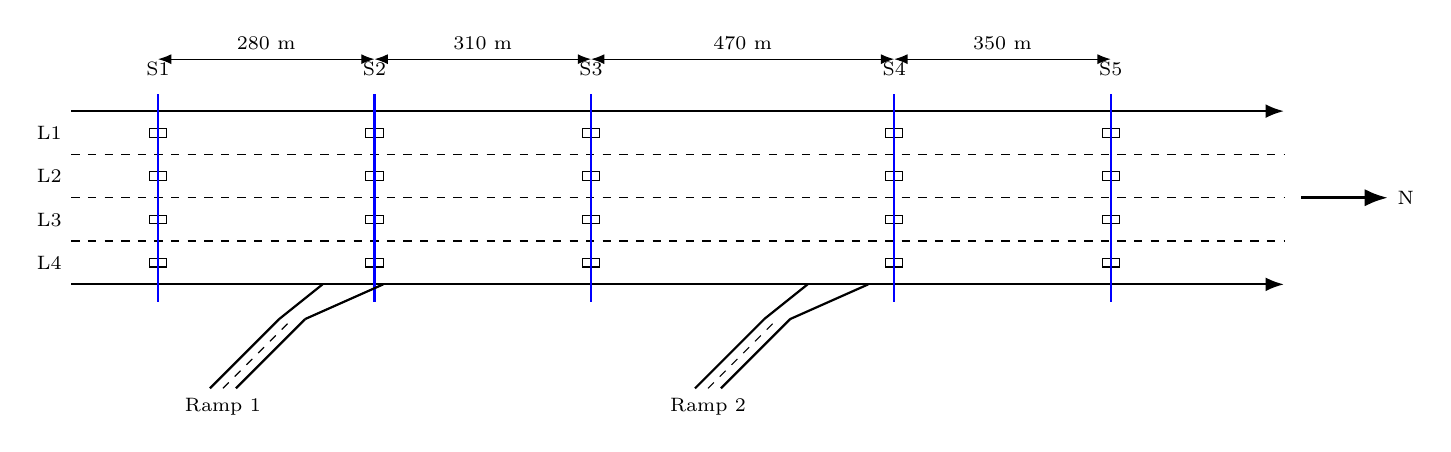
\begin{tikzpicture}[scale=1.1, >=Latex]

% ---- Road boundaries (ONLY these are solid) ----
            \draw[thick,->] (0,0) -- (14,0);     % bottom boundary
            \draw[thick,->] (0,2.0) -- (14,2.0); % top boundary

% ---- Lane separators (dashed) ----
            \foreach \y in {0.5,1.0,1.5} {
                \draw[dashed] (0,\y) -- (14,\y);
            }

% ---- Lane labels ----
            \node[left] at (0,1.75) {\scriptsize L1};
            \node[left] at (0,1.25) {\scriptsize L2};
            \node[left] at (0,0.75) {\scriptsize L3};
            \node[left] at (0,0.25) {\scriptsize L4};

% % ---- Central lane square markers ----
% \foreach \y in {1.75,1.25,0.75,0.25} {
%     \draw[fill=white] (0.3,\y-0.05) rectangle (0.5,\y+0.05);
% }

% ---- Rectangular boxes at each sensor (one per lane) ----
            \foreach \x in {1,3.5,6,9.5,12} {
                \foreach \y in {1.75,1.25,0.75,0.25} {
                    \draw[fill=white] (\x-0.1,\y-0.05) rectangle (\x+0.1,\y+0.05);
                }
            }


% ---- Sensors ----
            \foreach \x/\lab in {1/S1,3.5/S2,6/S3,9.5/S4,12/S5} {
                \draw[blue, thick] (\x,-0.2) -- (\x,2.2);
                \node[above] at (\x,2.3) {\scriptsize \lab};
            }

% ---- On-ramp 1 (two boundaries + dashed center) ----
            \draw[thick] (1.6,-1.2) -- (2.4,-0.4);
            \draw[thick] (1.9,-1.2) -- (2.7,-0.4);
            \draw[dashed] (1.75,-1.2) -- (2.55,-0.4);
% Open merge throat (separate endpoints)
% \draw[thick] (2.4,-0.4) -- (3.0,0.0);
% \draw[thick] (2.7,-0.4) -- (3.4,0.0);
            \draw[thick] (2.4,-0.4) -- (2.9,0.0);
            \draw[thick] (2.7,-0.4) -- (3.6,0.0);


            \node[below] at (1.75,-1.2) {\scriptsize Ramp 1};

% ---- On-ramp 2 (two boundaries + dashed center) ----
            \draw[thick] (7.2,-1.2) -- (8.0,-0.4);
            \draw[thick] (7.5,-1.2) -- (8.3,-0.4);
            \draw[dashed] (7.35,-1.2) -- (8.15,-0.4);
% \draw[thick] (8.0,-0.4) -- (8.8,0.0);
% \draw[thick] (8.3,-0.4) -- (8.8,0.0);
% Open merge throat for On-ramp 2
            \draw[thick] (8.0,-0.4) -- (8.5,0.0);
            \draw[thick] (8.3,-0.4) -- (9.2,0.0);

            \node[below] at (7.35,-1.2) {\scriptsize Ramp 2};


% ---- Distance annotations ----
            \draw[<->] (1,2.6) -- (3.5,2.6);
            \node[above] at (2.25,2.6) {\scriptsize 280 m};

            \draw[<->] (3.5,2.6) -- (6,2.6);
            \node[above] at (4.75,2.6) {\scriptsize 310 m};

            \draw[<->] (6,2.6) -- (9.5,2.6);
            \node[above] at (7.75,2.6) {\scriptsize 470 m};

            \draw[<->] (9.5,2.6) -- (12,2.6);
            \node[above] at (10.75,2.6) {\scriptsize 350 m};

% ---- Direction arrow ----
            \draw[very thick,->] (14.2,1.0) -- (15.2,1.0);
            \node[right] at (15.2,1.0) {\scriptsize N};

        \end{tikzpicture}
        \caption{Study corridor: US-101 northbound, Donald Doyle Highway segment, San Francisco. Five mainline loop detector stations (S1--S5) monitor four lanes. Two on-ramps merge between S1--S2 and S3--S4.}
        \label{fig:corridor}
    \end{figure}

    \subsection{Study Corridor}
    We model a 1.4 km segment of northbound US-101 in the Donald Doyle Highway area  near Danville, California (Figure~\ref{fig:corridor}). The corridor features four mainline lanes with two on-ramp merge points. Five loop detector stations are positioned along the mainline at approximately 280m, 310m, 470m, and 350m intervals, providing flow and speed measurements.
    The physical layout follows Figure 1 above. This corridor exhibits recurring congestion
    during morning and evening peak periods, making it suitable for validating car-following model calibration at the micro level.
    \subsection{Empirical Data}
    Traffic data was obtained from the California Performance Measurement System (PeMS),
    which collects real-time data from inductive loop detectors across California's freeway network. For the study corridor, we collected data from five mainline Vehicle Detector Stations (VDS 401112, 401104, 400712, 400450, and 407463) and two on-ramp detectors (VDS 403157 and 403108).

    Following the data processing approach of \cite{bowman2022microscopic}, the raw PeMS
    data recorded at 5-minute intervals was aggregated to 15-minute intervals to reduce
    noise while preserving congestion dynamics. This yields 48 time periods per simulation
    day (6:00 AM to 6:00 PM).
%To obtain representative weekday traffic patterns, we
% collected data from three consecutive weekdays (Tuesday, Wednesday, Thursday) and
% computed the average flow and speed for each lane and time interval. Weekend and
% holiday data were excluded to focus on recurring commute patterns.

    Each mainline detector provides lane-level measurements, yielding 20 flow time series
    (5 sensors $\times$ 4 lanes) and 20 speed time series for validation. Speed data
    recorded in mph was converted to m/s for simulation consistency. With 48 time
    intervals per series, the validation dataset comprises 1,920 data points per
    simulation day. On-ramp demand is derived from two single-lane ramp detectors,
    providing boundary conditions for merge traffic.

    All data underwent quality checks as outlines in \cite{law2007simulation} \cite{sargent2020verification} \cite{balci1995principles}. Sensor 4 lanes 2--3 exhibited anomalous speed readings (likely detector malfunction) (Need to continue this part)

    \subsection{Simulation Model}
    Our simulation is implemented in ScalaTion 2.0 \cite{miller2010using} \cite{miller2017advanced}, a Scala-based modeling and simulation framework. Scalation is a complete analytic suite built end to end to with scientific comoutation, simulation, result testing and validation. One may select different modeling paramdigm in Scalation such as Agent based, Process based or event based. In the work, our selected selective Scalation architecture follows a process-oriented discrete-event paradigm where each vehicle is an independent coroutine-based actor \cite{miller2017advanced} with the following key components:

    \begin{itemize}
        \item \textbf{MultiVSource:} Generates vehicles per lane using a suit of arrival process. We choose the Shifted Erlang-2 arrivals with data-driven mean inter-arrival times computed from PeMS flow data at each 15-minute interval for this work.
        \item \textbf{Pathway/Route:} Represents highway segments as doubly-linked lane structures supporting lane changes.
        \item \textbf{Dynamics:} Computes various selected Car following models,  IDM acceleration and integrates vehicle state using Dormand-Prince (DOPRI5) with adaptive step control.
        \item \textbf{Junction (Sensors):} Records vehicle counts and speeds at segment boundaries, aggregating to 15-minute intervals for comparison with PeMS data.
    \end{itemize}

    The simulation clock runs for 43,200 seconds (12 hours), with vehicles entering according to the time-varying arrival schedule derived from sensor 1 flow data.
    \subsection{Calibration and Optimization}

    Traffic microsimulation presents a noisy, non-convex optimization surface where
    gradient-based methods often fail due to stochastic simulation outputs and
    discontinuous lane-change events. We therefore employ derivative-free optimization
    to calibrate the IDM parameters governing car-following behavior.

    The calibration objective is to minimize the discrepancy between observed PeMS
    sensor data and simulated outputs. Let $\boldsymbol{\theta} = (s_0, a, b, T, \tau)$
    denote the parameter vector. The optimization problem is formulated as:

    \begin{equation}
        \boldsymbol{\theta}^* = \arg\min_{\boldsymbol{\theta} \in \Theta} \mathcal{L}(\boldsymbol{\theta})
    \end{equation}

    where $\Theta$ defines the bounded parameter space and $\mathcal{L}$ is the loss function.

    \begin{table}[h]
        \centering
        \caption{IDM Parameter Configuration}
        \begin{tabular}{|l|c|c|c|c|}
            \hline
            Parameter & Symbol & Unit & Bounds & Initial \\
            \hline
            Minimum gap & $s_0$ & m & [2.0, 8.0] & 5.0 \\
            Max acceleration & $a$ & m/s$^2$ & [1.5, 6.0] & 4.0 \\
            Comfortable deceleration & $b$ & m/s$^2$ & [1.0, 3.0] & 2.0 \\
            Safe time headway & $T$ & s & [1.0, 5.0] & 3.0 \\
            Reaction time & $\tau$ & s & [0.3, 1.5] & 0.5 \\
            \hline
        \end{tabular}
        \label{tab:idm_params}
    \end{table}

    Initial parameter values were selected based on exploratory runs that yielded stable simulation behavior. Parameter bounds were imposed to prevent the optimizer from exploring physically unrealistic regions following the approach of \cite{bowman2022microscopic}.

    \subsubsection{Loss function design.} Calibrating car-following models on a single
    measure of performance (MoP) can lead to Pareto-inefficient solutions: optimizing
    for speed alone degrades flow accuracy, and vice versa \cite{punzo2021calibration}.
    Following recommendations by Kesting and Treiber \cite{kesting2008calibrating} for
    joint speed-flow calibration, we define a balanced loss function using Normalized
    RMSE (NRMSE):

    \begin{equation}
        \text{NRMSE} = \frac{\text{RMSE}}{\bar{y}} = \frac{1}{\bar{y}} \sqrt{\frac{1}{n} \sum_{i=1}^{n} (y_i - \hat{y}_i)^2}
    \end{equation}

    where $\bar{y}$ is the mean of observed values. Normalization renders the metric
    dimensionless, enabling meaningful combination of speed and flow errors. The
    composite loss function is:

    \begin{equation}
        \mathcal{L}(\boldsymbol{\theta}) = 0.5 \cdot \text{NRMSE}_{\text{flow}} + 0.5 \cdot \text{NRMSE}_{\text{speed}}
    \end{equation}

    This equal weighting ensures neither flow counts nor speeds dominate the objective,
    avoiding calibration bias toward one measure at the expense of the other.

    \subsubsection{Optimizer selection.} We employ the Simultaneous Perturbation Stochastic
    Approximation (SPSA) algorithm \cite{spall2002implementation}, which estimates
    gradients using only two function evaluations per iteration regardless of parameter
    dimensionality. This efficiency is critical given our 40-minute simulation runtime
    per evaluation. SPSA iteratively updates parameters as:

    \begin{equation}
        \boldsymbol{\theta}_{k+1} = \boldsymbol{\theta}_k - a_k \hat{g}_k(\boldsymbol{\theta}_k)
    \end{equation}

    where $\hat{g}_k$ is the gradient estimate obtained by perturbing all parameters
    simultaneously with a random direction vector $\boldsymbol{\Delta}_k$.





    \section{RESULTS AND VALIDATION}
    \label{sec:results}
    \subsection{Macro-Level Validation}
    \subsection{Micro-Level Validation}

    \subsection{Discussion}


    \section{CONCLUSIONS}
    \label{sec:conclusions}

    \subsection{Toward digital twin}

% Use \verb+\cite+ to cite references in the \LaTeX source document. For example,

% \begin{verbatim}
%     \cite{law:simulationc,cheng:queuehetero}
% \end{verbatim} % no space after the comma!

% results in the citation~\cite{law:simulationc,cheng:queuehetero}.

% %There are a number of macros available to cite references in the \LaTeX\ source document.  The \verb+\cite+ macro can be used to give a list of references in parentheses.  For example,

% %\begin{verbatim}
% %\cite{law:simulationc,cheng:queuehetero}
% %\end{verbatim} % no space after the comma!

% %results in the citation~\cite{law:simulationc,cheng:queuehetero}. A reference that functions as a noun is created with the \verb+\citeN+ macro. For example,

% %\begin{verbatim}
% %\citeN{law:simulationc} say \ldots
% %\end{verbatim}

% %results in:~\citeN{law:simulationc} say \ldots\,.

% %Citations within parentheses do not need the extra parentheses provided by the above citation commands. To suppress the inclusion of extra parentheses, use the \verb+\citeNP+ macro. To obtain (\citeNP{cheng:queuehetero}, \citeNP{law:simulationc}), for example, use:

% %\begin{verbatim}
% %(\citeNP{cheng:queuehetero}, \citeNP{law:simulationc}).
% %\end{verbatim}

% %When there are four or more authors, the name of the first author should be given along with the text ``et al.''  This can be achieved with the \verb+\shortcite+ macro. To obtain~\shortcite{bcnn:simulation}, for example, use:

% %\begin{verbatim}
% %\shortcite{bcnn:simulation}
% %\end{verbatim}

% %The macros \verb+\shortciteN+ and \verb+\shortciteNP+ are also available to obtain `et al.' when a citation with many authors is used as a noun.

% %When citing a reference inside a figure or table caption, please use \verb+\protect\cite+ sequence to avoid build errors.
% %}

% \subsection{Generate the Bibliography File}

% Run \texttt{PDFLaTeX} (or \LaTeX), then \BibTeX, and then \texttt{PDFLaTeX} two more times. Running \texttt{PDFLaTeX} the first time creates the \texttt{.aux} file. Running \BibTeX\ creates the \texttt{.bbl} file.  Running \texttt{PDFLaTeX} again (twice) fixes the bibliography and citation references.


% \subsection{Include the Bibliography File in Your Submission}
% \label{sec:submitbib}

% \textcolor{red}{Be sure to include your \texttt{.bib} file(s) or your \texttt{.bbl} file as part of your submission}. If you only include the \texttt{.bbl} file, then please verify that you include the most up-to-date version reflecting changes during the editing process by rerunning \BibTeX\ one last time before submission.

% Please be aware that submitting the \texttt{.bbl} file instead of the \texttt{.bib} file means extra work for the editing team and for you, as any changes to the reference list need to be done by you in this case.
% Please open and save the file before every submission with software like JabRef to see whether the file is correct and to check for duplicated entries and/or bib keys in the file.


% \section{Author Checklist}
% We strive for a consistent appearance in all papers published in the proceedings. If you used the template and styles within this author’s kit, then almost all of the requirements in this checklist will be automatically satisfied, and there is very little to check.

% Please \textbf{print a hardcopy of your paper}, and go over your printed paper to make sure it adheres to the following requirements. \textit{Thank you!}
% \begin{enumerate}
% 	\item Abstract
%   \begin{enumerate}
% 	  \item \textcolor{red}{150 or fewer words.}
% 	  \item \textcolor{red}{Provide 3-5 keywords (mandatory).} This set of keywords will identify your paper in indices and databases.
% 	\end{enumerate}
% 	\item Paper Length
%   \begin{enumerate}
% 	  \item At least 5, but no more than 12 pages.
% 	  \item Page size is letter size (8.5’’ x 11’’, or 216 mm x 279 mm).
% 	\end{enumerate}
% 	\item All text is in 11-Point Times New Roman except the title, header, and footer (default in this template).
% 	\item Paper title is in 12-Point Times New Roman \textbf{BOLDFACE ALL CAPS} (default in this template).
% 	\item The paper has been \textcolor{red}{spellchecked using U.S. English}.
% 	\item Spacing and Margins
%   \begin{enumerate}
% 	  \item Single spaced.
% 	  \item Left and right margins are each 1 inch (default in this template).
% 	  \item Top and bottom margins are according to the template.
% 	  \item Title starts 1.25 inches from the top of the page (default in this template).
% 	\end{enumerate}
% 	\item Section Headings
%   \begin{enumerate}
% 	  \item Left justified and set in \textbf{BOLDFACE ALL CAPS} (default in this template).
% 	  \item Numbered, except for the abstract, acknowledgments, references, and author biographies.
% 	  \item Subsection headings are set in \textbf{Boldface Headline Style} (default in this template).
%     \item \textbf{Follow a logical order (\textbackslash section $\rightarrow$ \textbackslash subsection $\rightarrow$ \textbackslash subsubsection); do    not skip levels}.
% 	\end{enumerate}
% 	\item No footnotes or page numbers.
% %	\item The copyright notice on the first page contains the name of the symposium or a track where you want to submit your paper, and the running head on subsequent pages is the surnames of all authors.
% 	\item Multiple authors are formatted correctly.
% 	\item Equations are centered and any equation numbers are in parentheses and right-justified (default). \textbf{After key equations, add a one-sentence plain-language explanation in the surrounding text.}
% 	\item Figures and Tables
%   \begin{enumerate}
% 	  \item All text in figures and tables is readable.
%     \item Provide descriptive captions that explain the point of the visual;    do not rely on color alone to convey meaning.
%     \item Ensure sufficient color contrast ($\ge$4.5:1 for normal text;         $\ge$3:1 for large text).
% 	  \item Table captions appear above the table.
% 	  \item Figure captions appear below the figure.
% 	\end{enumerate}
% 	\item Citations and References
%   \begin{enumerate}
% 	  \item \textcolor{red}{Citations are by numbers between brackets} (default \BibTeX).
% 	  \item References are in the hangref style and are listed in the order they are cited in the text (also default \BibTeX\ setting in this template).
% 	\end{enumerate}
% 	\item Author biographies are one paragraph per author.
% 	\item Hyperlinks
%   \begin{enumerate}
% 	  \item Be sure that hyperlinks will probably work in the future as well.
% 	  \item Live hyperlinks are blue. Nonlive hyperlinks are black (default in this template).
%     \item \textbf{Use descriptive link text (e.g., “Conference website”) rather than only raw URLs.}
% 	\end{enumerate}
% 	\item All fonts must be embedded in the resulting \texttt{.pdf}. If you use \texttt{pdflatex}, this should already be true--unless you included figures in the \texttt{.eps} or \texttt{.pdf} format which may introduce additional font dependencies. You can use the \texttt{pdffonts} command to see if all the fonts are embedded (the column ``emb'' should say yes for all rows). You can use GhostScript to force embed the fonts, like so: {\texttt{gs -dNOPAUSE -dBATCH -sDEVICE=pdfwrite -dEmbedAllFonts=true -sOutputFile=out.pdf -f in.pdf}} (in Windows, use \texttt{gswin32} or \texttt{gswin32c} to invoke GhostScript).
% \end{enumerate}
% After verifying that your paper meets these requirements, please go to the final submission page at the conference website and submit your paper. Be sure to complete the transfer of copyright form and upload the \texttt{.pdf} receipt. \textit{Thank you for contributing to the SCS conferences!}


    \section*{Acknowledgments}

    Place the acknowledgments section, if needed, after the main text, but before any appendices and references. The section heading is not numbered. These instructions are adapted from the version by Roeder, T. M. K., Frazier, P. I., Wotton, H., Szechtman, R., Yooh, H. L., Harker, J., and Zhou, E. Those instructions were adapted from WSC instructions with permission from WSC BoD~\cite{WSC} that have been iteratively updated and improved by proceedings editors and several other individuals, who are too numerous to name separately since the first set of instructions were written by Barry Nelson for the 1991 WSC.

    \appendix

    \section{Appendices} \label{app:quadratic}
    Place any appendices after the acknowledgments. Note that the default style labels them A, B, C, and so forth (please, do not change this).
    The solution to \eqref{eq:quadratic} has the form:

    \begin{equation} \label{eq:quadratic sol}
        x = \frac{-b \pm \sqrt{b^2-4ac}}{2a} \mbox{ if } a \ne 0\;.
    \end{equation}

% Please don't change the bibliographystyle style
    \bibliographystyle{scsproc}

% AUTHOR: Include your bib file here
    \bibliography{assets/myReference}

    \section*{Author Biographies}

% \textbf{\uppercase{Korede R. Bishi}} is a third-year Computer Science Ph.D. student at the University of Georgia working in the Modeling, Simulation and Analytics Lab (MSAL) under the supervision of Dr. John A. Miller. My research centers on lane-level traffic simulation, trustworthy AI, and digital twins that adapt to urban mobility dynamics in real time. \email{korede.bishi@uga.edu}.

    \textbf{\uppercase{Casey Bowman}} Casey Bowman is a Professor of Mathematics at the University of North Georgia.  He earned his PhD in Computer Science from the University of Georgia in 2022.  His research interests include agent-based simulation, microscopic traffic simulation, calibration of simulation models, and simulation optimization \email{casey.bowman@ung.edu}.

% \textbf{\uppercase{John A. Miller}} is a Professor of Computer Science at the University of Georgia. He has been the Associate Head for 6 years and is/has been Graduate Coordinator for 13 years. His research interests include Modeling Simulation, Web Services/Workflow, Database Systems, and Big Data/Data Science. Dr. Miller received a B.S. in Applied Mathematics from Northwestern University in 1980 and an M.S. and Ph.D. in Information and Computer Science from the Georgia Institute of Technology in 1982 and 1986, respectively. In his areas of interest, Dr. Miller has authored over 200 research papers. He has served as General/Program Chair for four international research conferences: ANSS, WSC, ICWS, and SCC, as well as one regional research conference ACM-SE. \email{jamill@uga.edu}.


\end{document}
